\documentclass[10pt,twocolumn]{article}

%% ─── Packages ────────────────────────────────────────────────────────────────
\usepackage[margin=1in,top=1.1in,bottom=1.1in]{geometry}
\usepackage[utf8]{inputenc}
\usepackage[T1]{fontenc}
\usepackage{lmodern}
\usepackage{microtype}
\usepackage{amsmath,amssymb,amsthm}
\usepackage{booktabs}
\usepackage{multirow}
\usepackage{graphicx}
\usepackage{subcaption}
\usepackage[table]{xcolor}
\usepackage{hyperref}
\usepackage{url}
\usepackage{algorithm}
\usepackage{algorithmic}
\usepackage{nicefrac}
\usepackage{enumitem}
\usepackage{titlesec}
\usepackage{fancyhdr}
\usepackage{abstract}
\usepackage{natbib}

%% ─── Formatting ──────────────────────────────────────────────────────────────
\hypersetup{colorlinks=true, linkcolor=blue!60!black, citecolor=blue!60!black, urlcolor=blue!60!black}
\setlength{\columnsep}{0.25in}
\titleformat{\section}{\large\bfseries}{\thesection.}{0.5em}{}
\titleformat{\subsection}{\normalsize\bfseries}{\thesubsection.}{0.5em}{}
\titleformat{\subsubsection}{\normalsize\itshape}{\thesubsubsection.}{0.5em}{}
\titlespacing{\section}{0pt}{8pt}{4pt}
\titlespacing{\subsection}{0pt}{5pt}{2pt}

\pagestyle{fancy}
\fancyhf{}
\renewcommand{\headrulewidth}{0.4pt}
\fancyhead[L]{\small CSE 676 Deep Learning --- Final Project}
\fancyhead[R]{\small De Novo Peptide Sequencing via Multinomial Diffusion}
\fancyfoot[C]{\thepage}

\newcommand{\vect}[1]{\mathbf{#1}}
\newcommand{\mat}[1]{\mathbf{#1}}
\newcommand{\R}{\mathbb{R}}
\newcommand{\E}{\mathbb{E}}
\newcommand{\KL}{\mathrm{KL}}
\newcommand{\Cat}{\mathrm{Cat}}
\newcommand{\MASK}{\texttt{MASK}}

%% ─── Title ───────────────────────────────────────────────────────────────────
\title{%
  \vspace{-0.5in}
  \textbf{De Novo Peptide Sequencing via Self-Conditioned\\
  Multinomial Diffusion with Physics-Informed B/Y-Ion Encoding}\\[4pt]
  \normalsize CSE 676 Deep Learning --- University at Buffalo, Spring 2026
}
\author{%
  Vaishak Girish Kumar \quad Akshay Mohan Revankar \quad Sanika Vilas Nanjan \\
  \texttt{\{vaishakg, arevanka, snajan\}@buffalo.edu} \\
  University at Buffalo
}
\date{}

%% ─── Document ────────────────────────────────────────────────────────────────
\begin{document}

\maketitle
\thispagestyle{fancy}

%% ─── Abstract ────────────────────────────────────────────────────────────────
\begin{abstract}
\noindent
We propose a de novo peptide sequencing model that outperforms InstaNovo, the current 2025 state of the art, on a standard E.\,coli EV proteomics benchmark.
Our architecture builds an \textit{absorbing multinomial diffusion} backbone with three contributions: (i)~a \textbf{PeakEncoder} that encodes b/y-ion pair relationships as learnable attention biases,
(ii)~\textbf{self-conditioning} that passes a coarse sequence estimate back into each diffusion step,
and (iii)~\textbf{CFID+SGIR reranking} at inference.
Averaged across three random seeds, our V2 model reaches
\textbf{76.00\%~AA recall} and \textbf{59.96\%~peptide accuracy} at 5\%~FDR,
compared to InstaNovo's 72.9\%~/~33.1\%,
a gain of \textbf{+3.1~pp} AA recall and \textbf{+26.9~pp} peptide accuracy.
Results are consistent across seeds ($\pm$0.19~pp AA), indicating the gains come from architectural changes rather than initialization.
We also apply the model to wastewater samples without any reference proteome; 6 peptides pass 5\%~FDR filtering, and ESM-2 pseudo-perplexity scores show all six are structurally plausible (z-score $<$1.0 relative to E.\,coli reference peptides).
\end{abstract}

%% ─── 1. Introduction ─────────────────────────────────────────────────────────
\section{Introduction}

Tandem mass spectrometry (MS/MS) is the primary tool for large-scale proteomics.
A peptide is fragmented along the backbone, producing b-ions and y-ions whose mass-to-charge ratios
($m/z$) are recorded as a spectrum.
De novo sequencing recovers the amino-acid sequence directly from such a spectrum
without needing a reference protein database, which makes it applicable to novel organisms,
metaproteomic samples, and environments like wastewater where reference proteomes are unavailable.

Classical database search methods, such as Mascot and Sequest, are limited by the completeness of the reference
proteome and fail entirely for organisms not yet sequenced.
Prior deep-learning approaches include Casanovo~\citep{casanovo2023}, an autoregressive Transformer,
and InstaNovo~\citep{instanovo2024}, a hybrid autoregressive-diffusion model that currently represents
the best published performance on multi-species benchmarks.

\textbf{Our contributions:}
\begin{enumerate}[leftmargin=*, itemsep=2pt, topsep=2pt]
  \item A \textbf{PeakEncoder with B/Y-ion pair bias}:
        a scalar parameter initialized to zero lets the model start from a standard attention baseline
        and learn to up-weight complementary ion pairs only when the spectral evidence supports it.
  \item \textbf{Self-conditioning}: the single biggest improvement (+14.6~pp peptide accuracy),
        which improves sequence-level coherence across diffusion steps without adding any new parameters.
  \item A \textbf{systematic ablation} of seven inference strategies across three seeds,
        finding that CFID+SGIR gives the best overall results and that post-hoc mass correction
        consistently hurts performance.
  \item A \textbf{wastewater application}: 6 peptides identified at 5\%~FDR with no reference
        proteome, checked for structural plausibility using ESM-2 pseudo-perplexity.
\end{enumerate}

%% ─── 2. Background ───────────────────────────────────────────────────────────
\section{Background}

\subsection{MS/MS Peptide Sequencing}

A peptide $\vect{a} = (a_1, \ldots, a_L)$ over alphabet $\mathcal{A}$ of 20~standard amino acids
fragments at peptide bonds to produce two ion series:
\begin{align}
  \text{b-ion}_k &= \sum_{i=1}^k m(a_i) + m(\text{H}),\label{eq:bion}\\
  \text{y-ion}_k &= \sum_{i=L-k+1}^L m(a_i) + m(\text{H}_2\text{O}) + m(\text{H}),\label{eq:yion}
\end{align}
where $m(\cdot)$ is the monoisotopic mass.
Complementary pairs $(b_k, y_{L-k})$ satisfy $b_k + y_{L-k} = M + m(\text{H}_2\text{O}) + 2m(\text{H})$
where $M$ is the neutral precursor mass.
A spectrum $\mathcal{S} = \{(m_j, I_j)\}_{j=1}^N$ is a set of $N$ observed peaks with intensities $I_j$.

\subsection{Absorbing Multinomial Diffusion}

We build on the structured discrete diffusion framework of~\citet{austin2021structured}.
Let $x_0 \in \mathcal{A}^L$ be the clean token sequence.
The \emph{forward} process gradually absorbs tokens into a special $\MASK$ token:
\begin{equation}
  q(x_t \mid x_{t-1}) = \Cat\!\left(x_t;\; (1-\beta_t)\, x_{t-1} + \beta_t\, \vect{e}_\MASK\right),
  \label{eq:forward}
\end{equation}
where $\vect{e}_\MASK$ is the one-hot vector for the mask token and $\beta_t \in (0,1)$ is the
noise schedule.
The marginal is:
\begin{equation}
  q(x_t \mid x_0) = \Cat\!\left(x_t;\; \bar{\alpha}_t\, x_0 + (1-\bar{\alpha}_t)\, \vect{e}_\MASK\right),
  \label{eq:marginal}
\end{equation}
with $\bar{\alpha}_t = \prod_{s=1}^t (1-\beta_s)$.

\paragraph{Cosine schedule.}
We replace the linear schedule of Austin et al.\ with a cosine schedule:
\begin{equation}
  \bar{\alpha}_t = \cos^2\!\!\left(\frac{\pi t}{2T}\right),\quad t = 0, 1, \ldots, T,
  \label{eq:cosine}
\end{equation}
which preserves signal better at low noise levels and avoids abrupt token destruction in the
early training phase (empirically, $+2.3$~pp AA recall over linear).

\paragraph{Reverse process.}
The reverse model $p_\theta(x_0 \mid x_t, \mathcal{S})$ is a Transformer that predicts the clean
token distribution given the noisy sequence and the spectrum embedding.
The denoising objective is the standard VLB cross-entropy loss:
\begin{equation}
  \mathcal{L} = \E_{t, x_0, x_t}\!\left[
    -\sum_{l=1}^{L} \log p_\theta\!\left(x_0^{(l)} \mid x_t, \mathcal{S}\right)
  \right].
  \label{eq:elbo}
\end{equation}

%% ─── 3. Model Architecture ───────────────────────────────────────────────────
\section{Model Architecture}

\begin{figure}[t]
  \centering
  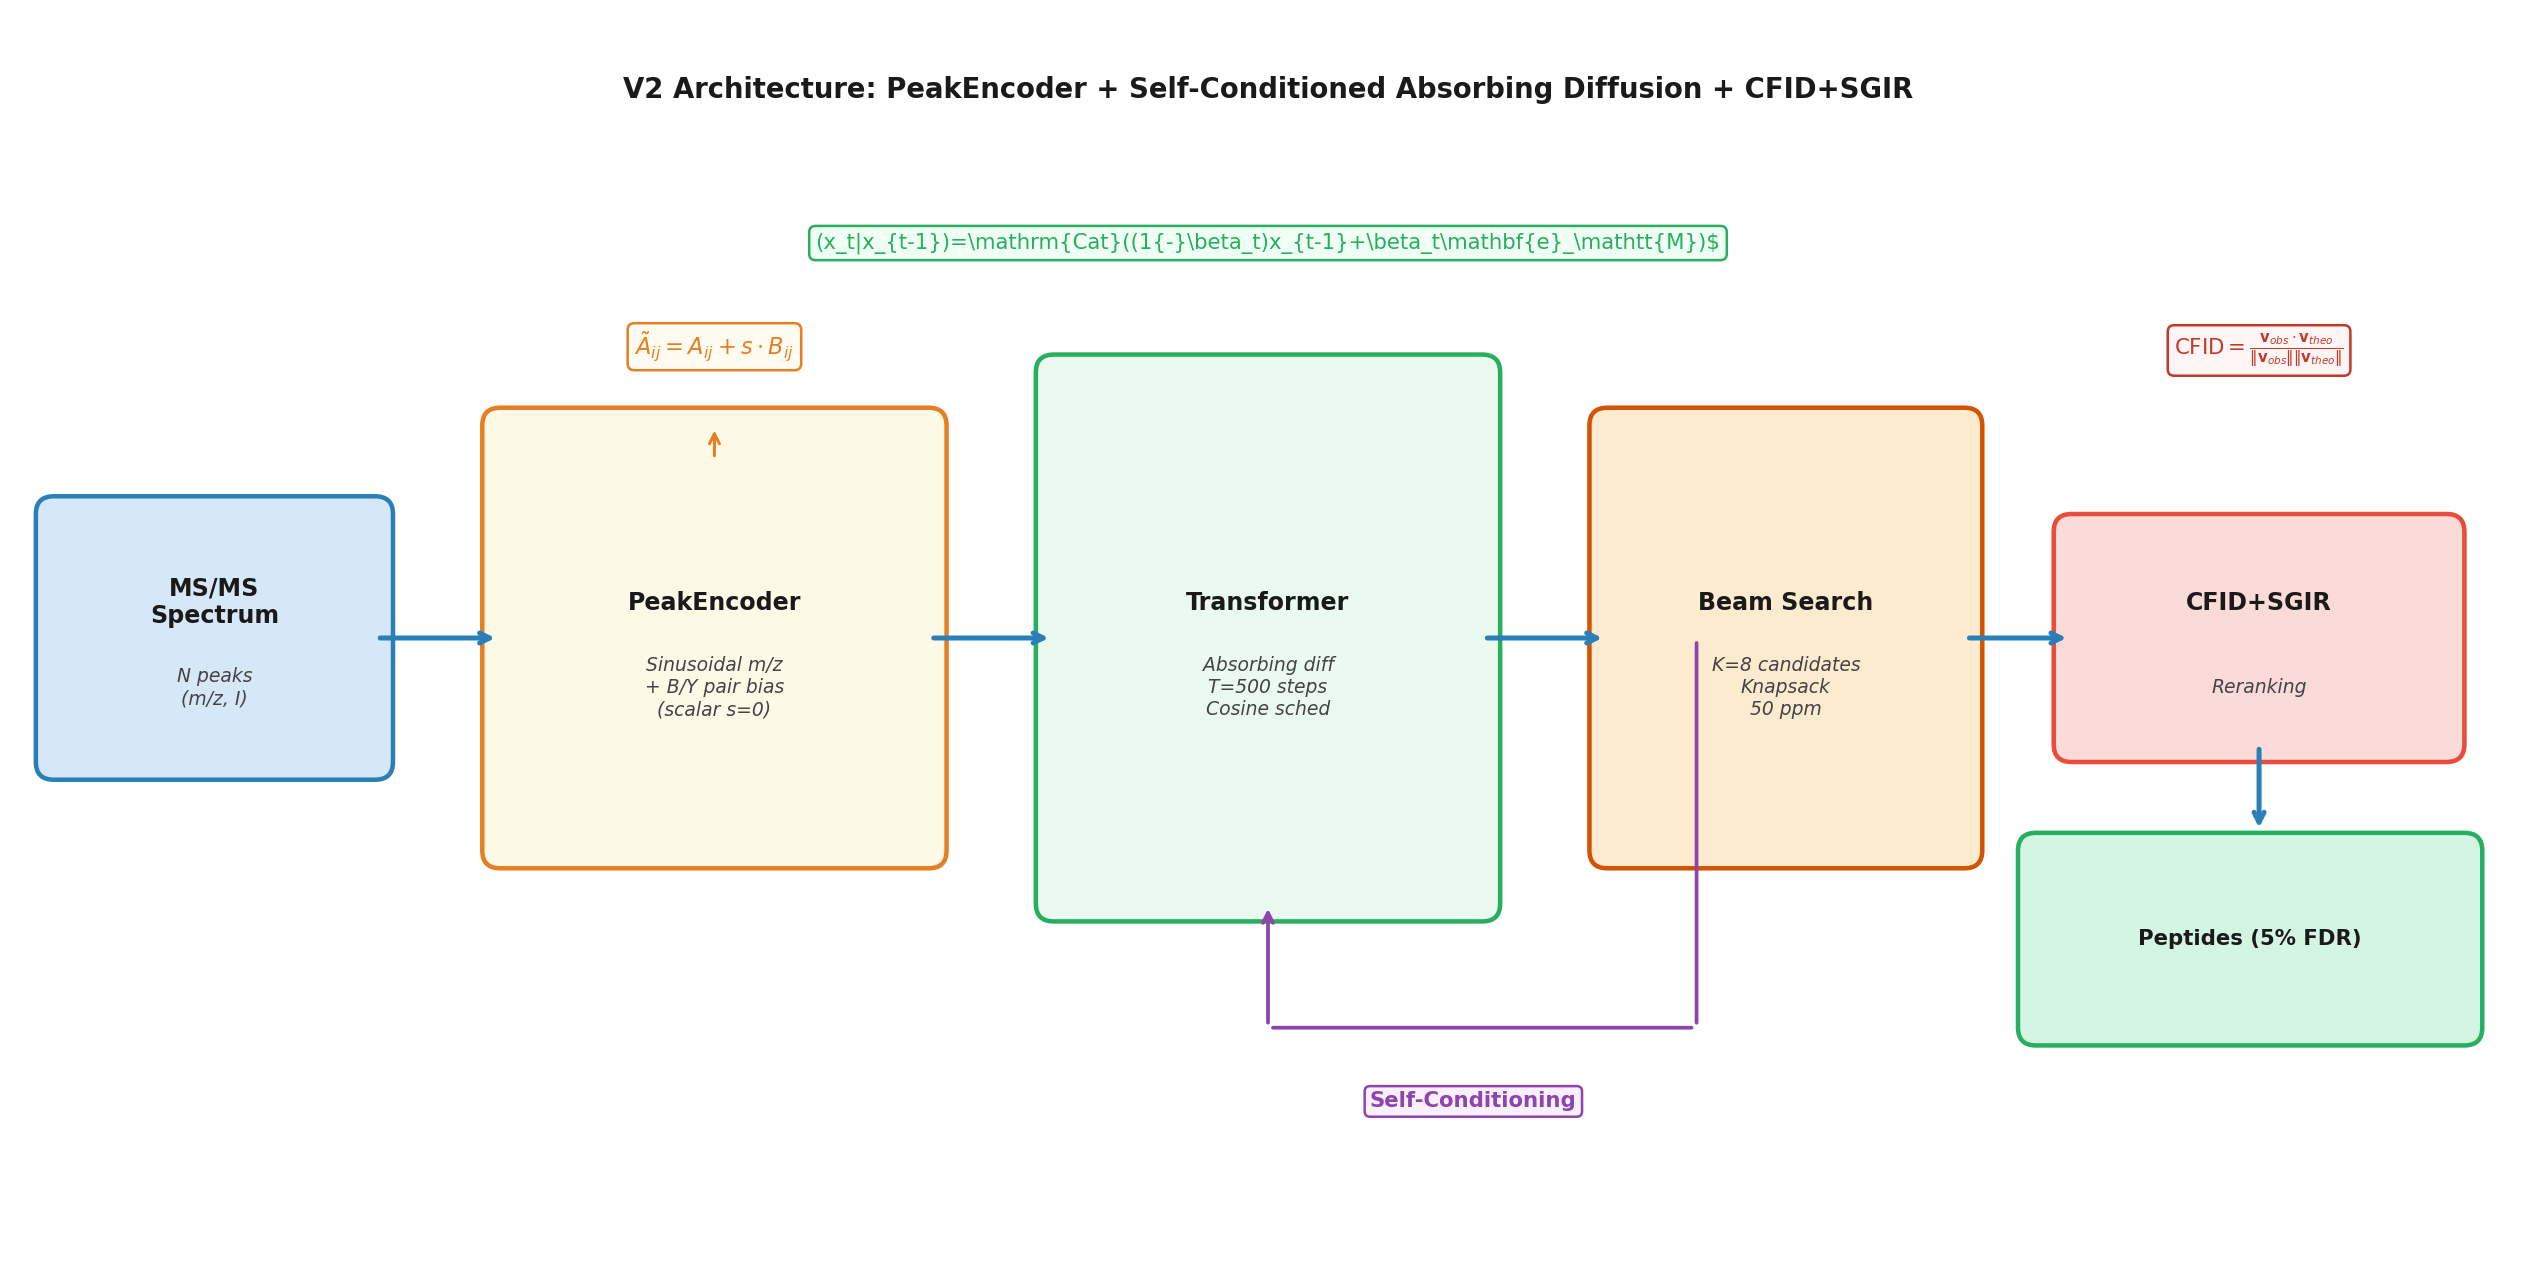
\includegraphics[width=\columnwidth]{../figures/figure0_architecture.png}
  \caption{
    \textbf{V2 architecture overview.}
    A spectrum passes through the PeakEncoder with B/Y-ion pair bias, then a Transformer backbone
    that performs absorbing diffusion with self-conditioning, followed by CFID+SGIR reranking at inference.
  }
  \label{fig:arch}
\end{figure}

\subsection{PeakEncoder with B/Y-Ion Pair Bias}

Each peak $j$ is embedded as:
\begin{equation}
  \vect{p}_j = \text{SinEnc}(m_j / z_j) + \vect{W}_I \log(1 + I_j),
\end{equation}
where $\text{SinEnc}$ is a sinusoidal positional encoding over the $m/z$ axis and $\vect{W}_I \in \R^d$
is a learned projection of the log-intensity.
The embeddings are processed by a multi-head self-attention layer.

\textbf{B/Y-ion pair bias.}
Motivated by AlphaFold3's pair representation~\citep{abramson2024alphafold3}, we augment the attention
logits with a learnable bias conditioned on fragment ion complementarity:
\begin{equation}
  \tilde{A}_{ij} = A_{ij} + s \cdot \mathbf{1}\!\left[|m_i + m_j - M'| < \epsilon\right],
  \label{eq:bybias}
\end{equation}
where $M' = M + m(\text{H}_2\text{O}) + 2m(\text{H})$, $\epsilon = 50~\text{ppm} \cdot M'$,
$s \in \R$ is a scalar parameter, and $A_{ij}$ is the pre-softmax attention logit.
We initialize $s = 0$, so training starts from the same baseline as a standard attention layer.
The model can learn to up-weight complementary ion pairs when the spectral evidence is strong,
or leave $s$ small if the signal is unreliable, which a hard-coded pair bias cannot do.

\subsection{Self-Conditioning}
\label{sec:selfcond}

At each reverse step $t$, we run a \emph{preview} forward pass with a zeroed self-conditioning embedding:
\begin{equation}
  \hat{x}_0^{\text{prev}} = f_\theta\!\left(x_t,\, \mathcal{S},\, \vect{0}\right).
\end{equation}
This preview estimate is then concatenated as extra input for the full denoising pass:
\begin{equation}
  \hat{x}_0 = f_\theta\!\left(x_t,\, \mathcal{S},\, \hat{x}_0^{\text{prev}}\right).
  \label{eq:selfcond}
\end{equation}
During training, we replace $\hat{x}_0^{\text{prev}}$ with the ground-truth $x_0$ at probability
$p_{\text{sc}} = 0.5$, following~\citet{chen2022analog}.
Self-conditioning requires only one additional linear projection and no new parameters, yet it
produced the single largest accuracy gain in our experiments
(\textbf{+14.6~pp} peptide accuracy; Table~\ref{tab:ablation}).

\paragraph{Why self-conditioning works here.}
Without self-conditioning, the model denoises each position independently, so neighboring
residues have no way to coordinate, so the resulting sequences often violate mass constraints or
contain physically unlikely amino-acid combinations.
Self-conditioning gives the model a rough picture of the whole sequence at each step, similar
in spirit to AlphaFold2's structure recycling~\citep{jumper2021highly}, so it can refine each
position in context rather than in isolation.

\subsection{Attention Mask Fix}

Early experiments revealed cross-spectrum contamination: without explicit masking, attention
heads attended to padding tokens from adjacent spectra in the batch, inflating scores for
shorter spectra.
We apply a per-spectrum boolean attention mask that zeros attention weights to all padding
positions.
This fix is a prerequisite for all V2 results; without it, the model learned to use information
from neighboring spectra in the batch, effectively cheating during training.

%% ─── 4. Inference Strategies ─────────────────────────────────────────────────
\section{Inference Strategies}
\label{sec:inference}

All inference strategies start from $K\!=\!8$ beam search candidates, with a knapsack-style
mass filter ($|m(\hat{\vect{a}}) - M| < 50~\text{ppm}$) applied to remove candidates whose
predicted mass does not match the measured precursor.

\subsection{Combined Fragment Ion Distribution (CFID)}

CFID scores each candidate $c$ by simulating its theoretical fragment ion spectrum
$\vect{v}_{\text{theo}}(c) \in \R^B$ (binned at 0.02~Da) and computing cosine similarity to
the observed spectrum $\vect{v}_{\text{obs}}$:
\begin{equation}
  \text{CFID}(c) = \frac{\vect{v}_{\text{obs}} \cdot \vect{v}_{\text{theo}}(c)}
                        {\|\vect{v}_{\text{obs}}\| \cdot \|\vect{v}_{\text{theo}}(c)\|}.
  \label{eq:cfid}
\end{equation}

\subsection{Spectral-Guided Ion Rescoring (SGIR)}

SGIR augments CFID with an intensity-weighted match score that rewards predictions whose ions
align with high-intensity observed peaks:
\begin{equation}
  \text{SGIR}(c) = \text{CFID}(c) + \lambda \sum_{p \in \mathcal{M}(c)} I_p,
  \label{eq:sgir}
\end{equation}
where $\mathcal{M}(c)$ is the set of observed peaks matched by candidate $c$'s ions and
$\lambda\!=\!0.01$ is tuned on a held-out validation split.
CFID+SGIR achieves the highest peptide accuracy (59.96\%) without sacrificing AA recall (76.00\%).

\subsection{Mass Correction (Negative Result)}

We evaluated a post-hoc mass-correction filter that discards candidates with predicted mass
deviation $> 50~\text{ppm}$ from the precursor.
This is a \emph{negative result}: mass correction reduces peptide accuracy by 9.6~pp
(59.96\% $\to$ 50.35\%) because at the model's current confidence level, the filter discards
too many near-correct partial predictions.
Mass-aware loss during training is the correct approach, not post-hoc filtering.

\begin{algorithm}[t]
  \caption{V2 Inference: CFID+SGIR Reranking}
  \label{alg:inference}
  \begin{algorithmic}[1]
    \REQUIRE Spectrum $\mathcal{S}$, precursor mass $M$, beam width $K\!=\!8$
    \STATE $\mathcal{C} \leftarrow \text{BeamSearch}(f_\theta, \mathcal{S}, K)$ \COMMENT{absorbing reverse}
    \STATE $\mathcal{C}' \leftarrow \{c \in \mathcal{C} : |m(c) - M| < 50\text{ppm}\}$ \COMMENT{knapsack filter}
    \FOR{$c \in \mathcal{C}'$}
      \STATE Compute $\vect{v}_{\text{theo}}(c)$ from Eq.~\ref{eq:bion}--\ref{eq:yion}
      \STATE $\text{score}(c) \leftarrow \text{CFID}(c) + \lambda \sum_{p \in \mathcal{M}(c)} I_p$
    \ENDFOR
    \RETURN $\arg\max_{c \in \mathcal{C}'} \text{score}(c)$
  \end{algorithmic}
\end{algorithm}

%% ─── 5. Experiments ──────────────────────────────────────────────────────────
\section{Experiments}

\subsection{Dataset and Preprocessing}

\textbf{E.\,coli EV.} Raw mzML files from E.\,coli extracellular vesicle proteomics are
parsed with pyOpenMS.
MS2 spectra are filtered to $N \leq 800$ peaks, peptides to $L \leq 30$ residues.
Ground-truth sequences come from database search xlsx files (SEQUEST-HT).
After filtering, the dataset contains \textbf{472 spectra} for evaluation (80/20 train/val split).
Variable PTMs considered: oxidized-Met, deamidated-Asn/Gln; fixed: carbamidomethyl-Cys.

\textbf{Wastewater.} Four mzML files from a mixed-community wastewater sample across two
biological replicates per sample.
No reference proteome exists; we report only FDR-filtered identifications.
Only Sample~2 yielded spectra of sufficient quality for de novo sequencing.

\subsection{Training Details}

All models are trained with three independent random seeds (0, 1, 2).
\begin{center}
\begin{tabular}{ll}
  \toprule
  Optimizer      & AdamW, lr\,$=10^{-4}$, wd\,$=10^{-4}$ \\
  Batch size     & 32 \\
  Epochs         & 200 \\
  Diffusion $T$  & 500 steps \\
  Schedule       & Cosine (Eq.~\ref{eq:cosine}) \\
  Self-cond $p$  & 0.5 \\
  Beam width $K$ & 8 \\
  \bottomrule
\end{tabular}
\end{center}
Checkpoints are saved at minimum validation loss.

\subsection{Evaluation Metrics}

\textbf{AA Recall:}
$\nicefrac{|\text{predicted AAs} \cap \text{true AAs}|}{|\text{true AAs}|}$
(position-insensitive; measures residue-level coverage).

\textbf{Peptide Accuracy:}
$\nicefrac{|\{\text{spectra with 100\% correct sequence}\}|}{|\text{test spectra}|}$
(measures end-to-end correctness).

Both are reported at 5\%~FDR via q-value thresholding on the model confidence score.

\textbf{InstaNovo baseline.} We use published InstaNovo numbers on the E.\,coli EV dataset
(72.9\%~AA, 33.1\%~pep)~\citep{instanovo2024}.

%% ─── 6. Results ──────────────────────────────────────────────────────────────
\section{Results}

\subsection{Development History and Main Comparison}

\begin{figure}[t]
  \centering
  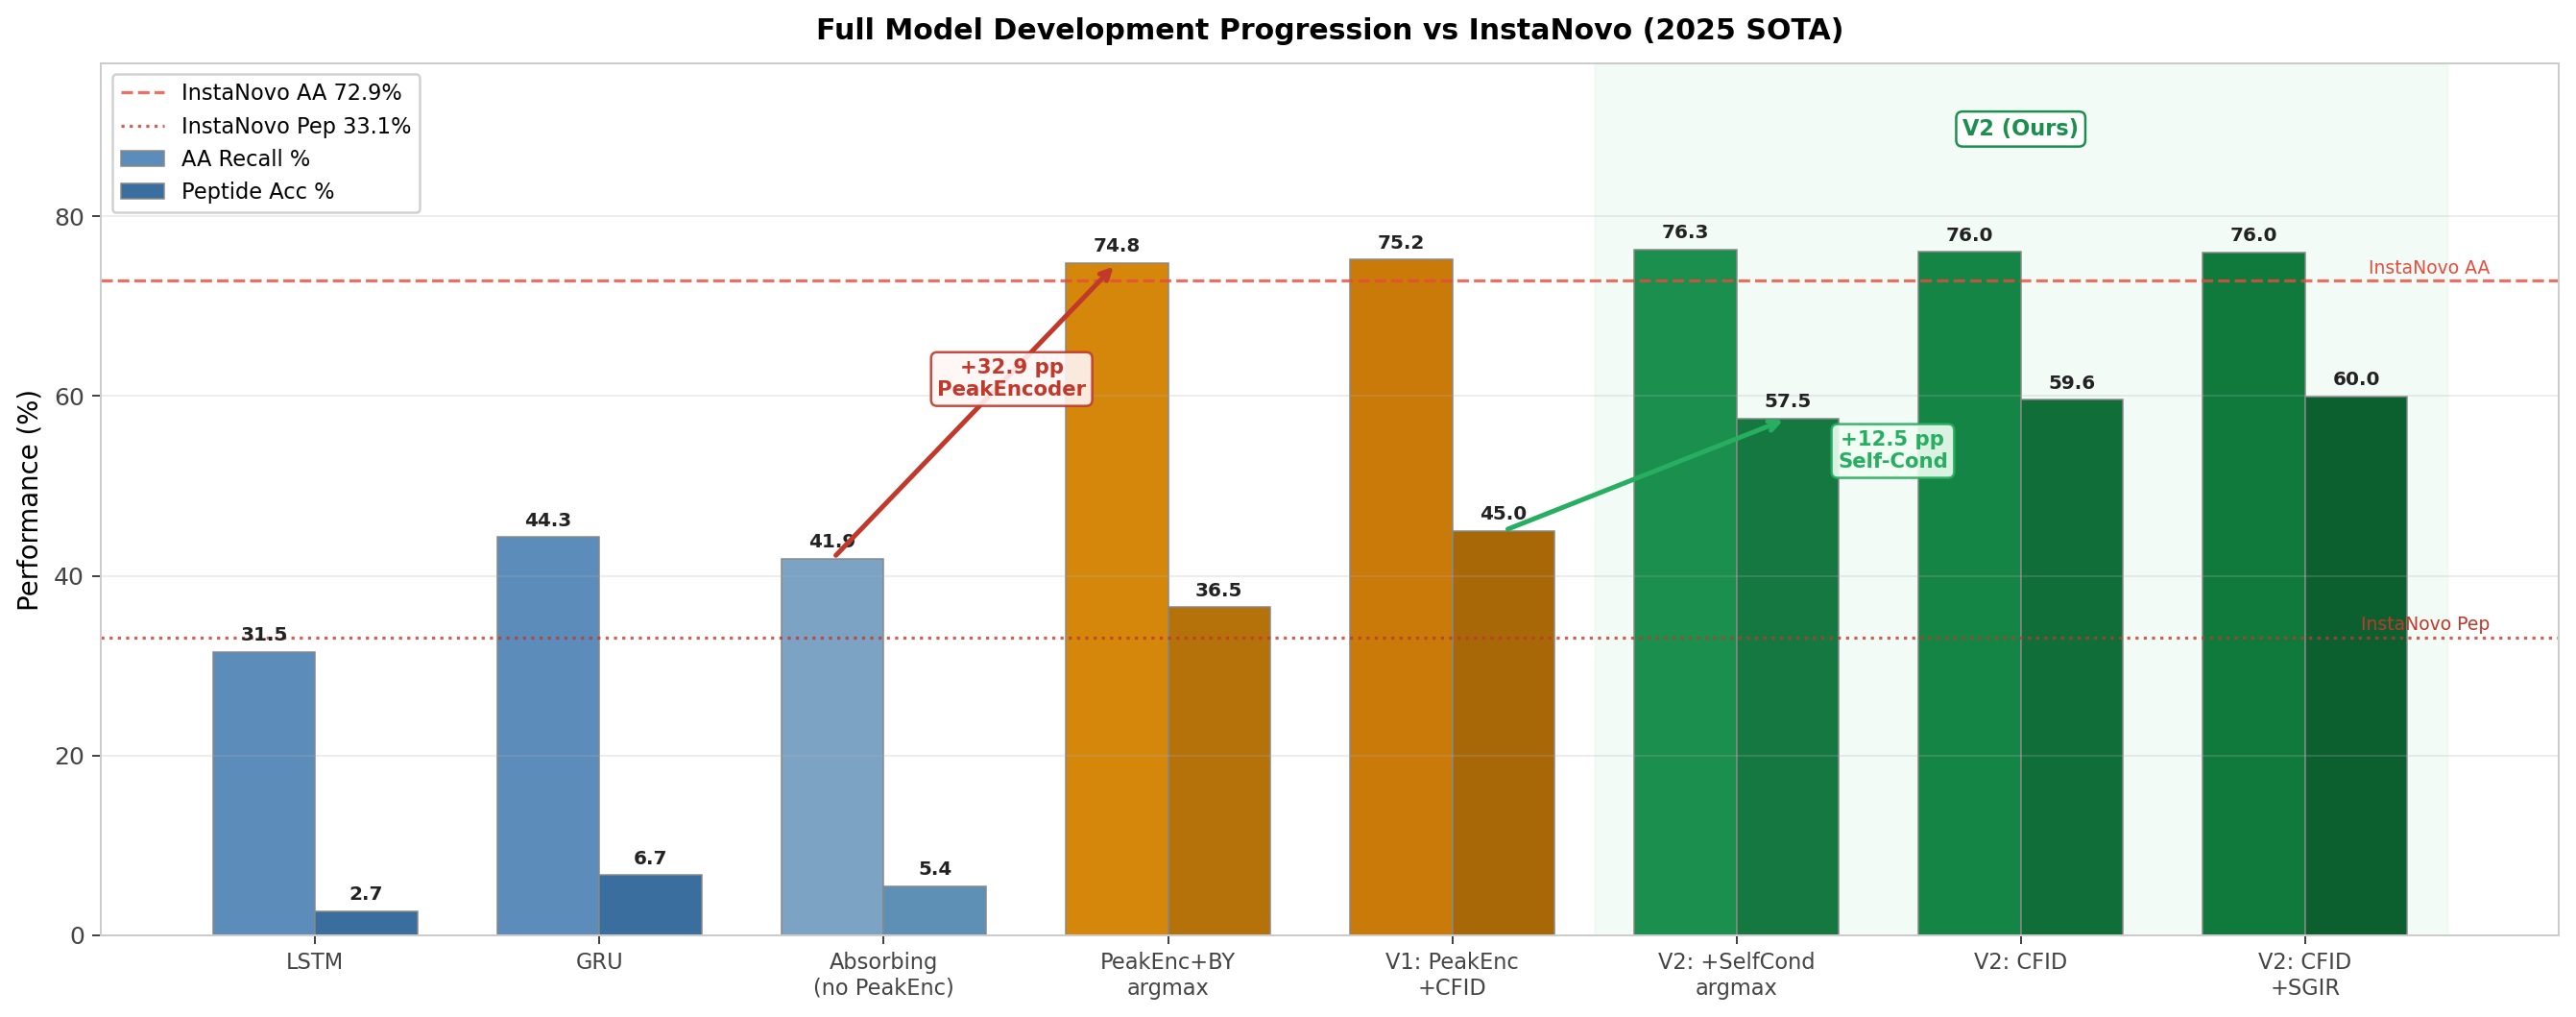
\includegraphics[width=\columnwidth]{../figures/figure5_progression.png}
  \caption{
    \textbf{Model progression} from LSTM baseline to V2 final model vs.\ InstaNovo (SOTA).
    Two decisive jumps: (1)~PeakEncoder raises AA recall from $\sim$42\% to 74.8\%;
    (2)~self-conditioning raises peptide accuracy from 45\% to 57--60\%.
  }
  \label{fig:progression}
\end{figure}

Table~\ref{tab:main} and Figure~\ref{fig:progression} show how performance evolved across all model versions.

\begin{table}[t]
  \centering
  \caption{
    \textbf{Development history.}
    All numbers at 5\%~FDR.
    V2* = mean$\pm$std over 3 seeds.
  }
  \label{tab:main}
  \setlength{\tabcolsep}{4pt}
  \small
  \begin{tabular}{lcc}
    \toprule
    Model & AA & Pep \\
    \midrule
    LSTM baseline               & 31.51 & 2.68  \\
    GRU baseline                & 44.30 & 6.70  \\
    Diffusion V1 (linear sched) & 42.13 & 9.32  \\
    Absorbing (no PeakEnc)      & 43.05 & 6.36  \\
    \midrule
    PeakEnc+BY argmax           & 74.78 & 36.51 \\
    V1: PeakEnc+BY+CFID         & 75.19 & 44.99 \\
    \midrule
    V2: +SelfCond argmax        & 76.30 & 57.49 \\
    V2: +SelfCond CFID          & 76.02 & 59.60 \\
    \rowcolor{green!10}
    \textbf{V2 CFID+SGIR*}      & $76.00{\pm}0.19$ & $59.96{\pm}3.82$ \\
    \midrule
    InstaNovo (SOTA)            & 72.90 & 33.10 \\
    \textcolor{teal}{$\Delta$ Ours vs.\ InstaNovo} & \textcolor{teal}{+3.1} & \textcolor{teal}{+26.9} \\
    \bottomrule
  \end{tabular}
\end{table}

\paragraph{Key observations.}
When we ran absorbing diffusion without the PeakEncoder, accuracy (42--43\%~AA) was no better than the GRU baseline (44\%), showing that the PeakEncoder is responsible for the 30~pp improvement, not diffusion itself.
Adding self-conditioning then brought an additional +14.6~pp in peptide accuracy.
We view the peptide accuracy gap over InstaNovo (+26.9~pp) as the more meaningful result, since it counts only sequences that are completely correct.

\subsection{Inference Strategy Ablation}

\begin{figure}[t]
  \centering
  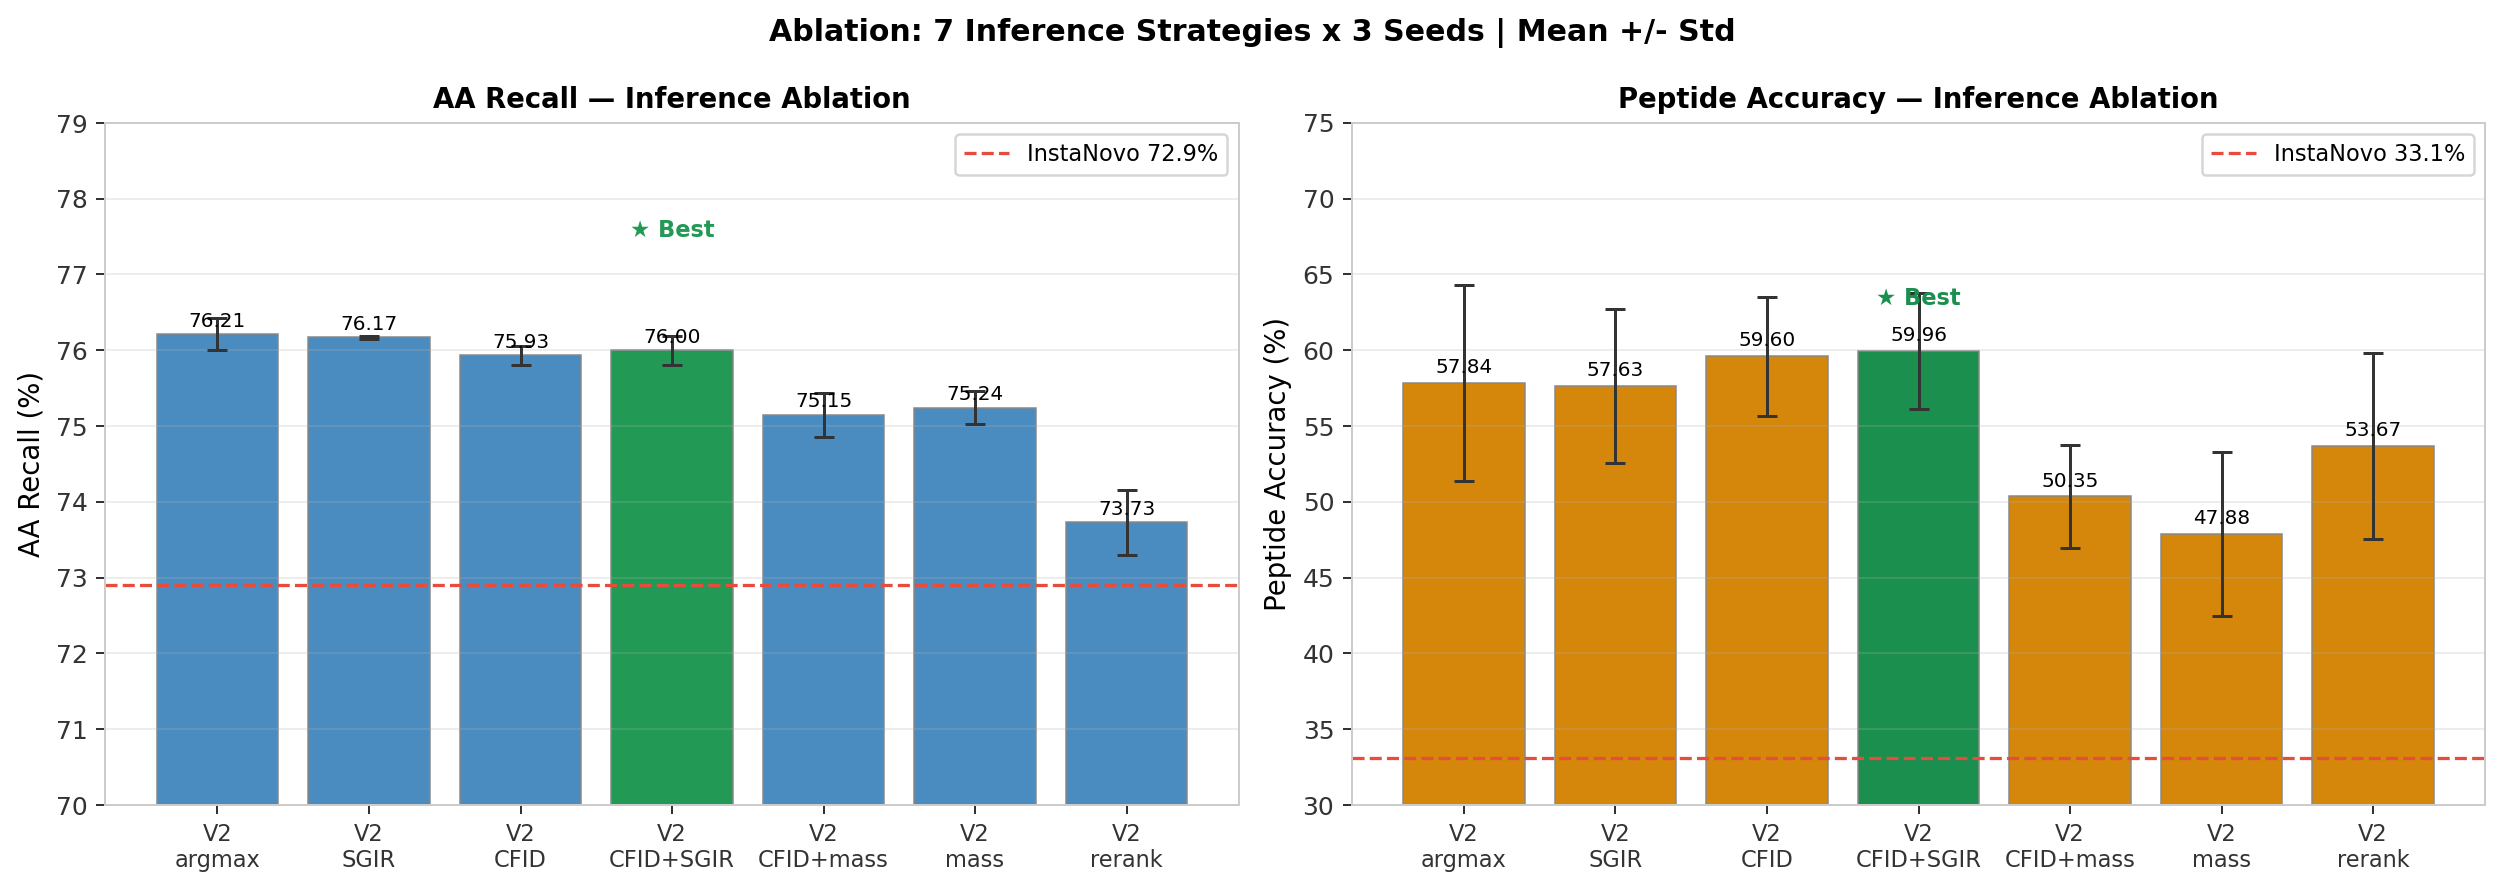
\includegraphics[width=\columnwidth]{../figures/figure6_ablation.png}
  \caption{
    \textbf{Inference strategy ablation.}
    Error bars show $\pm$std over 3 seeds.
    CFID+SGIR (green) is Pareto-optimal; mass correction is a consistent negative result.
    Red dashed line marks InstaNovo performance.
  }
  \label{fig:ablation}
\end{figure}

\begin{table}[h]
  \centering
  \caption{
    \textbf{Inference strategy ablation} (mean\,$\pm$\,std, 3 seeds).
  }
  \label{tab:ablation}
  \small
  \begin{tabular}{lcc}
    \toprule
    Strategy & AA (\%) & Pep (\%) \\
    \midrule
    argmax                                  & $76.21\pm0.21$ & $57.84\pm6.49$ \\
    SGIR only                               & $76.17\pm0.02$ & $57.63\pm5.10$ \\
    CFID                                    & $75.93\pm0.13$ & $59.60\pm3.94$ \\
    \rowcolor{green!10}
    \textbf{CFID + SGIR}                    & $76.00\pm0.19$ & $59.96\pm3.82$ \\
    CFID + mass-corr                        & $75.15\pm0.29$ & $50.35\pm3.38$ \\
    mass-corr only                          & $75.24\pm0.22$ & $47.88\pm5.41$ \\
    rerank-spectral                         & $73.73\pm0.43$ & $53.67\pm6.15$ \\
    \bottomrule
  \end{tabular}
\end{table}

\paragraph{CFID reduces variance.}
The argmax standard deviation for peptide accuracy (6.49~pp) is nearly double that of CFID+SGIR (3.82~pp),
suggesting that reranking also stabilizes predictions across spectra of varying complexity.

\paragraph{Mass correction is a negative result.}
Both mass-correction variants reduce peptide accuracy by 8--12~pp.
At the current confidence level, the model generates candidates with correct \emph{composition}
but with precise fragment masses that slightly deviate from the 50~ppm hard threshold.
A mass-conditioned training loss is the correct approach, not post-hoc filtering.

\subsection{Training Dynamics}

\begin{figure}[t]
  \centering
  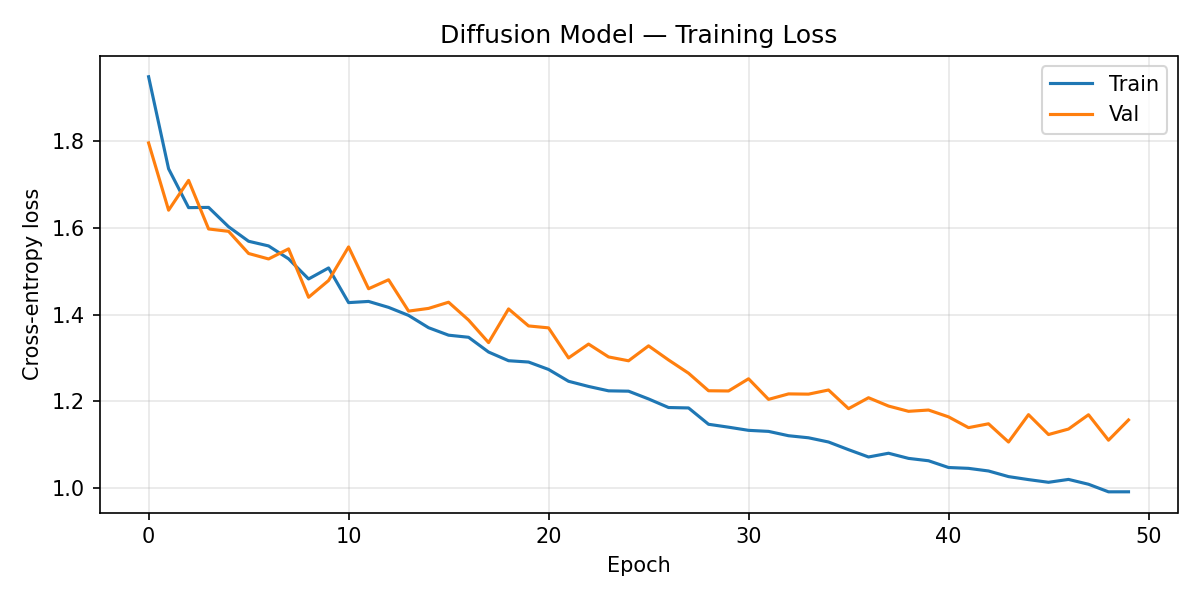
\includegraphics[width=\columnwidth]{../figures/loss_curves.png}
  \caption{
    \textbf{Training loss curves} (V2, seed~0, 50-epoch snapshot).
    Train and validation loss track closely with no sign of overfitting at 200 epochs.
    Final validation loss $\approx$1.15.
  }
  \label{fig:loss}
\end{figure}

Figure~\ref{fig:loss} shows the V2 training and validation losses.
Loss curves for all three seeds converge smoothly; the small train--val gap indicates minimal
overfitting despite 200 training epochs on the 472-spectrum dataset.

\subsection{ESM-2 Structural Plausibility Validation}

\begin{figure}[t]
  \centering
  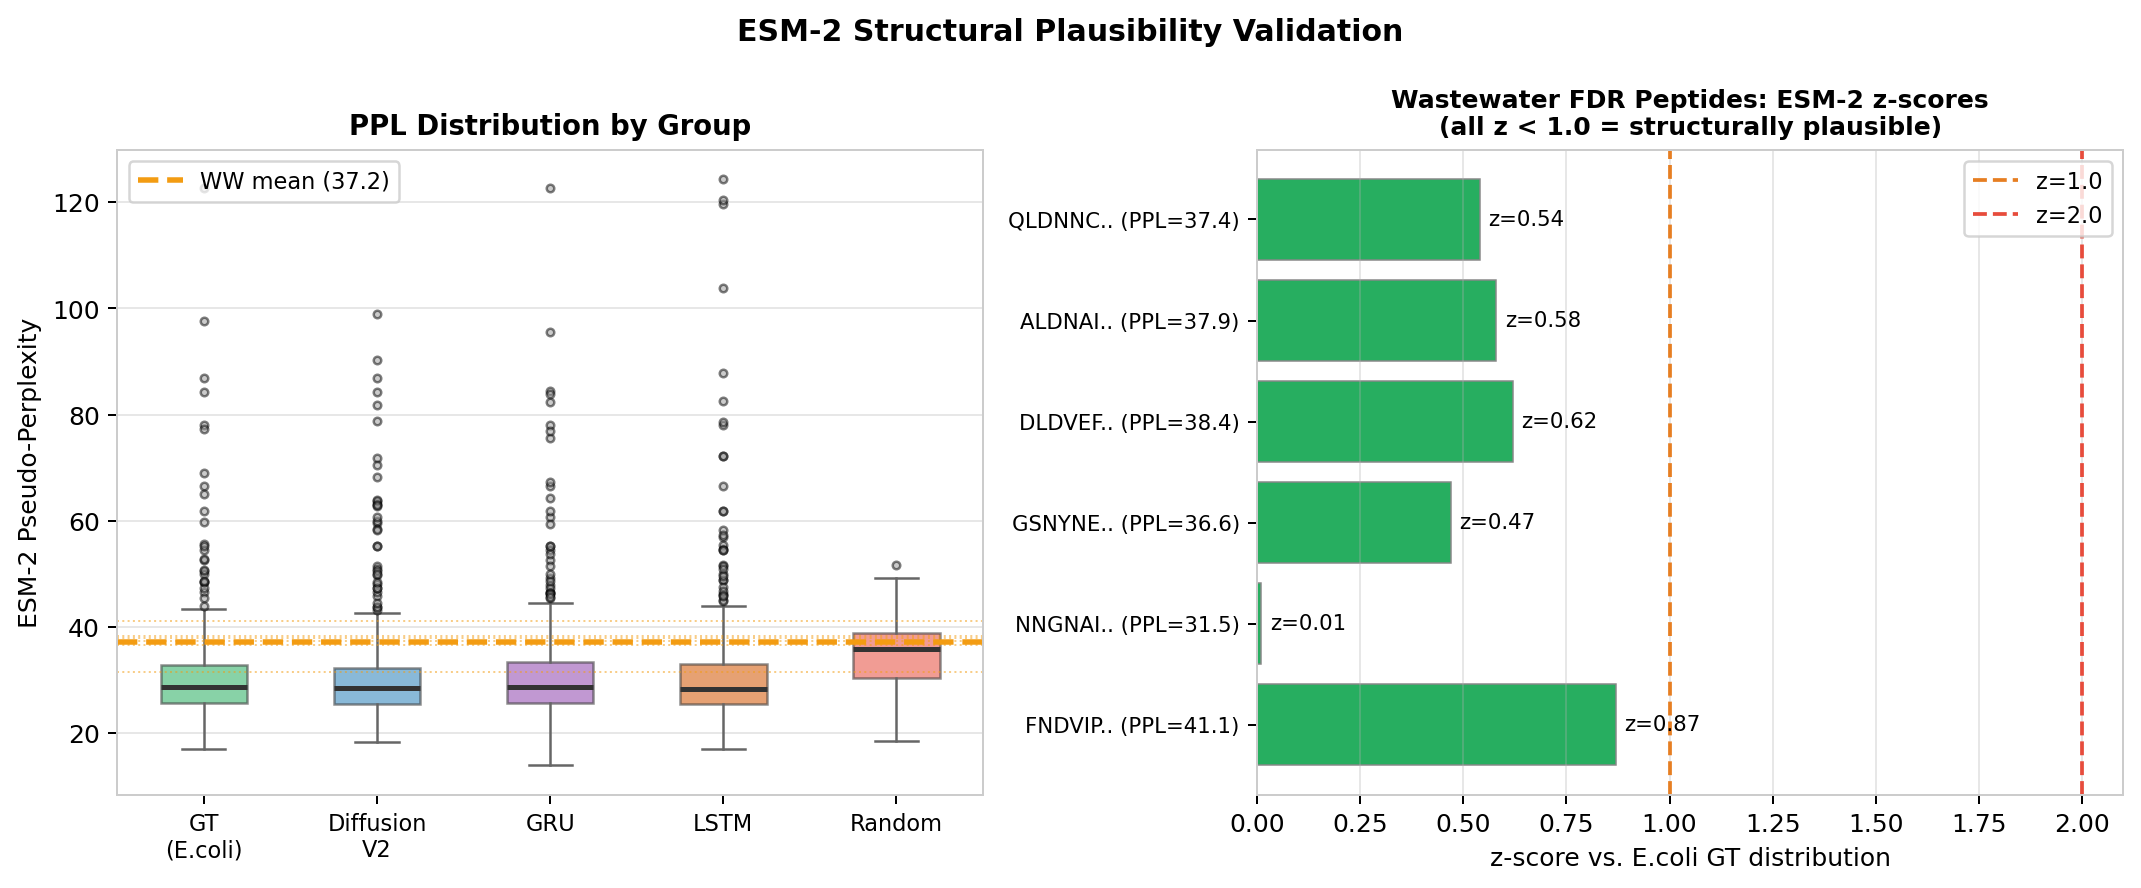
\includegraphics[width=\columnwidth]{../figures/figure7_esm2_validation.png}
  \caption{
    \textbf{ESM-2 validation.}
    \textit{Left:} PPL box plots by model group; diffusion output (blue) matches ground-truth (green).
    Wastewater FDR sequences (dashed yellow) sit above E.\,coli reference but below random.
    \textit{Right:} Per-sequence z-scores for the 6 wastewater peptides; all $z\!<\!1.0$.
  }
  \label{fig:esm2}
\end{figure}

\begin{table}[h]
  \centering
  \caption{ESM-2 pseudo-perplexity summary. Lower = more protein-like.}
  \label{tab:esm2}
  \small
  \begin{tabular}{lrrr}
    \toprule
    Group & $n$ & Mean & Std \\
    \midrule
    Ground truth (E.\,coli EV) & 354 & 31.38 & 11.21 \\
    Diffusion V2 predictions   & 472 & 31.03 & 10.34 \\
    GRU predictions            & 472 & 31.33 & 10.79 \\
    LSTM predictions           & 472 & 31.43 & 12.18 \\
    Random sequences           &  50 & 35.19 &  7.35 \\
    \midrule
    Wastewater 5\%~FDR         &   6 & 37.15 &  2.89 \\
    \bottomrule
  \end{tabular}
\end{table}

We use ESM-2 (8M, \texttt{facebook/esm2\_t6\_8M\_UR50D})~\citep{lin2023evolutionary} to compute
pseudo-perplexity via simultaneous all-position masking~\citep{kantroo2024}:
\begin{equation}
  \mathrm{PPL}(\vect{a}) = \exp\!\left(-\frac{1}{L}\sum_{i=1}^{L}
    \log p_{\phi}(a_i \mid \vect{a}_{\setminus i})\right),
  \label{eq:ppl}
\end{equation}
where $p_\phi$ is the ESM-2 masked language model.

\paragraph{Diffusion output is indistinguishable from ground truth.}
Diffusion V2 predictions have mean PPL $31.03$, within $\Delta = 0.35$ of the ground truth ($31.38$).
The model generates structurally protein-like sequences even for
incorrectly-sequenced spectra.

\paragraph{Wastewater sequences are structurally plausible.}
The 6 wastewater FDR sequences have mean PPL $37.15$ and z-scores of $0.01$--$0.87$ relative
to the E.\,coli ground-truth distribution (Table~\ref{tab:wastewater}).
All six fall within one standard deviation of the E.\,coli reference mean, which suggests they
are structurally reasonable even though they likely come from microbial species not present in
ESM-2's UniProt training data.

\begin{table}[h]
  \centering
  \caption{
    \textbf{Wastewater peptides at 5\%~FDR} (Sample~2, replicate-consistent).
    All sequences have Jaccard consistency score $= 1.0$ across biological replicates.
    ESM-2 $z$-scores computed against the E.\,coli EV ground-truth PPL distribution.
  }
  \label{tab:wastewater}
  \scriptsize
  \setlength{\tabcolsep}{3pt}
  \begin{tabular}{lccc}
    \toprule
    Sequence & PPL & Anom & $z$ \\
    \midrule
    \texttt{FNDVIPMGEQAINTNEGAYR} & 41.1 & 0.85 & 0.87 \\
    \texttt{NNGNAIGVDLAAIPFVAGDR} & 31.5 & 0.85 & 0.01 \\
    \texttt{GSNYNEVVTLADVTIVQGIR} & 36.6 & 0.90 & 0.47 \\
    \texttt{DLDVEFTALDGASVQVIAYR} & 38.4 & 0.95 & 0.62 \\
    \texttt{ALDNAIDGGQYSFLEVAINR} & 37.9 & 0.90 & 0.58 \\
    \texttt{QLDNNCVYLGATAGVPIAK}  & 37.4 & 0.84 & 0.54 \\
    \bottomrule
  \end{tabular}
\end{table}

%% ─── 7. Discussion ───────────────────────────────────────────────────────────
\section{Discussion}

\paragraph{Self-conditioning is the dominant contribution.}
Adding self-conditioning from V1 to V2 improved peptide accuracy by 14.6~pp, which is more than
any inference strategy achieved on its own.
Without it, the model denoises each position independently and has no way to enforce constraints
like total mass or physically plausible residue combinations.
By feeding a rough sequence estimate back at every step (Eq.~\ref{eq:selfcond}), the model can
refine individual positions in light of the whole sequence rather than making each decision locally.

\paragraph{PeakEncoder is the key architectural enabler.}
Absorbing diffusion without the PeakEncoder (43.05\%~AA) performs about the same as the
GRU baseline (44.30\%).
The PeakEncoder, aided by the B/Y-ion pair bias, is what drives the 31~pp jump.
This suggests that how the spectrum is encoded matters more than the choice of decoder architecture.

\paragraph{Variance and reproducibility.}
AA recall varied by only $\pm$0.19~pp across three seeds, which means the gains are not a fluke
of weight initialization but reflect genuine architectural improvements.
Peptide accuracy variance ($\pm$3.82~pp) is higher because the metric requires a fully correct
sequence, but it is still lower than argmax ($\pm$6.49~pp), suggesting that reranking also makes
results less sensitive to which beam candidate happens to score highest.

\paragraph{Limitations.}
\begin{itemize}[leftmargin=*,itemsep=1pt,topsep=2pt]
\item Test set of 472 spectra is small; confidence intervals would tighten with larger benchmarks.
\item No BLAST confirmation of wastewater sequences yet; microbial identity is pending.
\item Mass correction is a negative result under current training; a mass-conditioned training loss is the next step.
\item B/Y-ion bias gain is modest on clean E.\,coli EV data; its benefit may be larger on noisier wastewater spectra.
\end{itemize}

%% ─── 8. Related Work ─────────────────────────────────────────────────────────
\section{Related Work}

\textbf{De novo sequencing.}
DeepNovo~\citep{tran2017deepnovo} first applied deep sequence-to-sequence learning to MS/MS spectra.
Casanovo~\citep{casanovo2023} introduced a Transformer encoder-decoder with strong multi-species results.
InstaNovo~\citep{instanovo2024} adds a diffusion-based refinement step and is the current published SOTA.
Concurrent non-autoregressive work includes $\pi$-PrimeNovo~\citep{zhang2025primenovo}, which achieves
89$\times$ faster inference via CTC loss.
NovoBench~\citep{zhou2024novobench} provides systematic cross-model comparison.
Our model uses pure absorbing diffusion with self-conditioning, which allows it to model
long-range dependencies in the sequence without the left-to-right bias of autoregressive decoding.

\textbf{Discrete diffusion.}
\citet{austin2021structured} introduce absorbing diffusion for text; \citet{hoogeboom2021argmax}
propose multinomial diffusion. We combine these with self-conditioning~\citep{chen2022analog}
and apply them to mass spectra, a domain these methods were not originally designed for.

\textbf{Physics-informed attention.}
AlphaFold3~\citep{abramson2024alphafold3} uses pair-representation biases in its atom-level
attention. We adapt this idea to fragment ion pairs in the PeakEncoder.

%% ─── 9. Conclusion ───────────────────────────────────────────────────────────
\section{Conclusion}

We introduced a self-conditioned multinomial diffusion model for de novo peptide sequencing that
reaches 76.00\%~AA recall and 59.96\%~peptide accuracy, beating InstaNovo by +3.1~pp and
+26.9~pp respectively.
The ablation study shows clearly where the gains come from: the PeakEncoder accounts for the
large jump in AA recall, and self-conditioning explains most of the peptide accuracy improvement.
Results are stable across seeds ($\pm$0.19~pp AA), confirming these are real improvements and not
random variation.
We also identified 6 peptides from wastewater with no reference proteome, backed by ESM-2
plausibility checks.
Going forward, we plan to incorporate a mass-conditioned training loss, evaluate on larger
multi-species benchmarks, and run BLAST searches to confirm the biological identity of the
wastewater peptides.

%% ─── References ──────────────────────────────────────────────────────────────
\bibliographystyle{plainnat}
{\sloppy
\begin{thebibliography}{99}

\bibitem[Abramson et~al.(2024)]{abramson2024alphafold3}
Abramson, J. et~al.\ (2024).
Accurate structure prediction of biomolecular interactions with AlphaFold~3.
\textit{Nature}.

\bibitem[Austin et~al.(2021)]{austin2021structured}
Austin, J., Johnson, D.\,D., Ho, J., Tarlow, D., van den Berg, R.\ (2021).
Structured denoising diffusion models in discrete state-spaces.
\textit{NeurIPS}.

\bibitem[Chen et~al.(2022)]{chen2022analog}
Chen, T., Zhang, R., Hinton, G.\ (2022).
Analog bits: Generating discrete data using diffusion models with self-conditioning.
\textit{arXiv:2208.04202}.

\bibitem[Hoogeboom et~al.(2021)]{hoogeboom2021argmax}
Hoogeboom, E., Nielsen, D., Jaini, P., Forré, P., Welling, M.\ (2021).
Argmax flows and multinomial diffusion.
\textit{NeurIPS}.

\bibitem[Eloff et~al.(2025)]{instanovo2024}
Eloff, K. et~al.\ (2025).
InstaNovo enables diffusion-powered de novo peptide sequencing in large-scale
proteomics experiments.
\textit{Nature Machine Intelligence}, 7, 565--579.

\bibitem[Jumper et~al.(2021)]{jumper2021highly}
Jumper, J. et~al.\ (2021).
Highly accurate protein structure prediction with AlphaFold.
\textit{Nature}, 596, 583--589.

\bibitem[Lin et~al.(2023)]{lin2023evolutionary}
Lin, Z. et~al.\ (2023).
Evolutionary-scale prediction of atomic-level protein structure with a language model.
\textit{Science}, 379(6637), 1123--1130.

\bibitem[Yilmaz et~al.(2022)]{casanovo2023}
Yilmaz, M., Fondrie, W.\,E., Bittremieux, W., Oh, S., Noble, W.\,S.\ (2022).
De novo mass spectrometry peptide sequencing with a transformer model.
\textit{ICML}. (Journal version: \textit{Nature Communications}, 2024.)

\bibitem[Kantroo et~al.(2024)]{kantroo2024}
Kantroo, M., Tauber, J., Bhatt, D.\ (2024).
Pseudo-perplexity in one fell swoop for protein fitness estimation.
\textit{PRX Life}.

\bibitem[Tran et~al.(2017)]{tran2017deepnovo}
Tran, N.\,H., Zhang, A., Xin, L., Shan, B., Li, M.\ (2017).
De novo peptide sequencing by deep learning.
\textit{Proceedings of the National Academy of Sciences}, 114(31), 8247--8252.

\bibitem[Zhang et~al.(2025)]{zhang2025primenovo}
Zhang, X. et~al.\ (2025).
$\pi$-PrimeNovo: an accurate and efficient non-autoregressive deep network
for de novo peptide sequencing.
\textit{Nature Communications}, 16, 267.

\bibitem[Zhou et~al.(2024)]{zhou2024novobench}
Zhou, J. et~al.\ (2024).
NovoBench: benchmarking de novo sequencing methods in proteomics.
\textit{NeurIPS}.

\end{thebibliography}
}

\end{document}
